\section{Gradient Computation}
I managed to successfully write the functions to correctly compute the gradient analytically.
I tested my implementation by computing the gradients using both ComputeGradsNum.m and ComputeGradsNumSlow.m.
Then I compared my results with the numerical approaches by calculating the absolute difference of each gradient element as in equations below.
Then I checked those against a threshold (1e-5). 
When using the reduced set with \texttt{d=20} and \texttt{n=2} and using ComputeGradsNumSlow.m 
I get a maximum error of 
\begin{itemize}
    \item \texttt{diff\_W1\_max = 3.9846e-11}
    \item \texttt{diff\_b1\_max = 2.9749e-11}
    \item \texttt{diff\_W2\_max = 3.3175e-11}
    \item \texttt{diff\_b2\_max = 3.2699e-11}
\end{itemize}
Using ComputeGradsNum.m I get 
\begin{itemize}
    \item \texttt{diff\_W1\_max = 1.9299e-07}
    \item \texttt{diff\_b1\_max = 1.3112e-07}
    \item \texttt{diff\_W2\_max = 6.4177e-07}
    \item \texttt{diff\_b2\_max = 5.6976e-07}
\end{itemize}
These errors are small enough to conclude that my implementation works. \\ 
\begin{equation}\label{eq:diffw}
    diff\_W = abs(ngrad\_W - grad\_W)
\end{equation}
\begin{equation}\label{eq:diffb}
    diff\_b = abs(ngrad\_b - grad\_b)
\end{equation}
\\
After that I trained the network with 100 examples, \texttt{lambda=0} for 200 epochs, which resulted in overfitting:
    \begin{figure}[ht]
        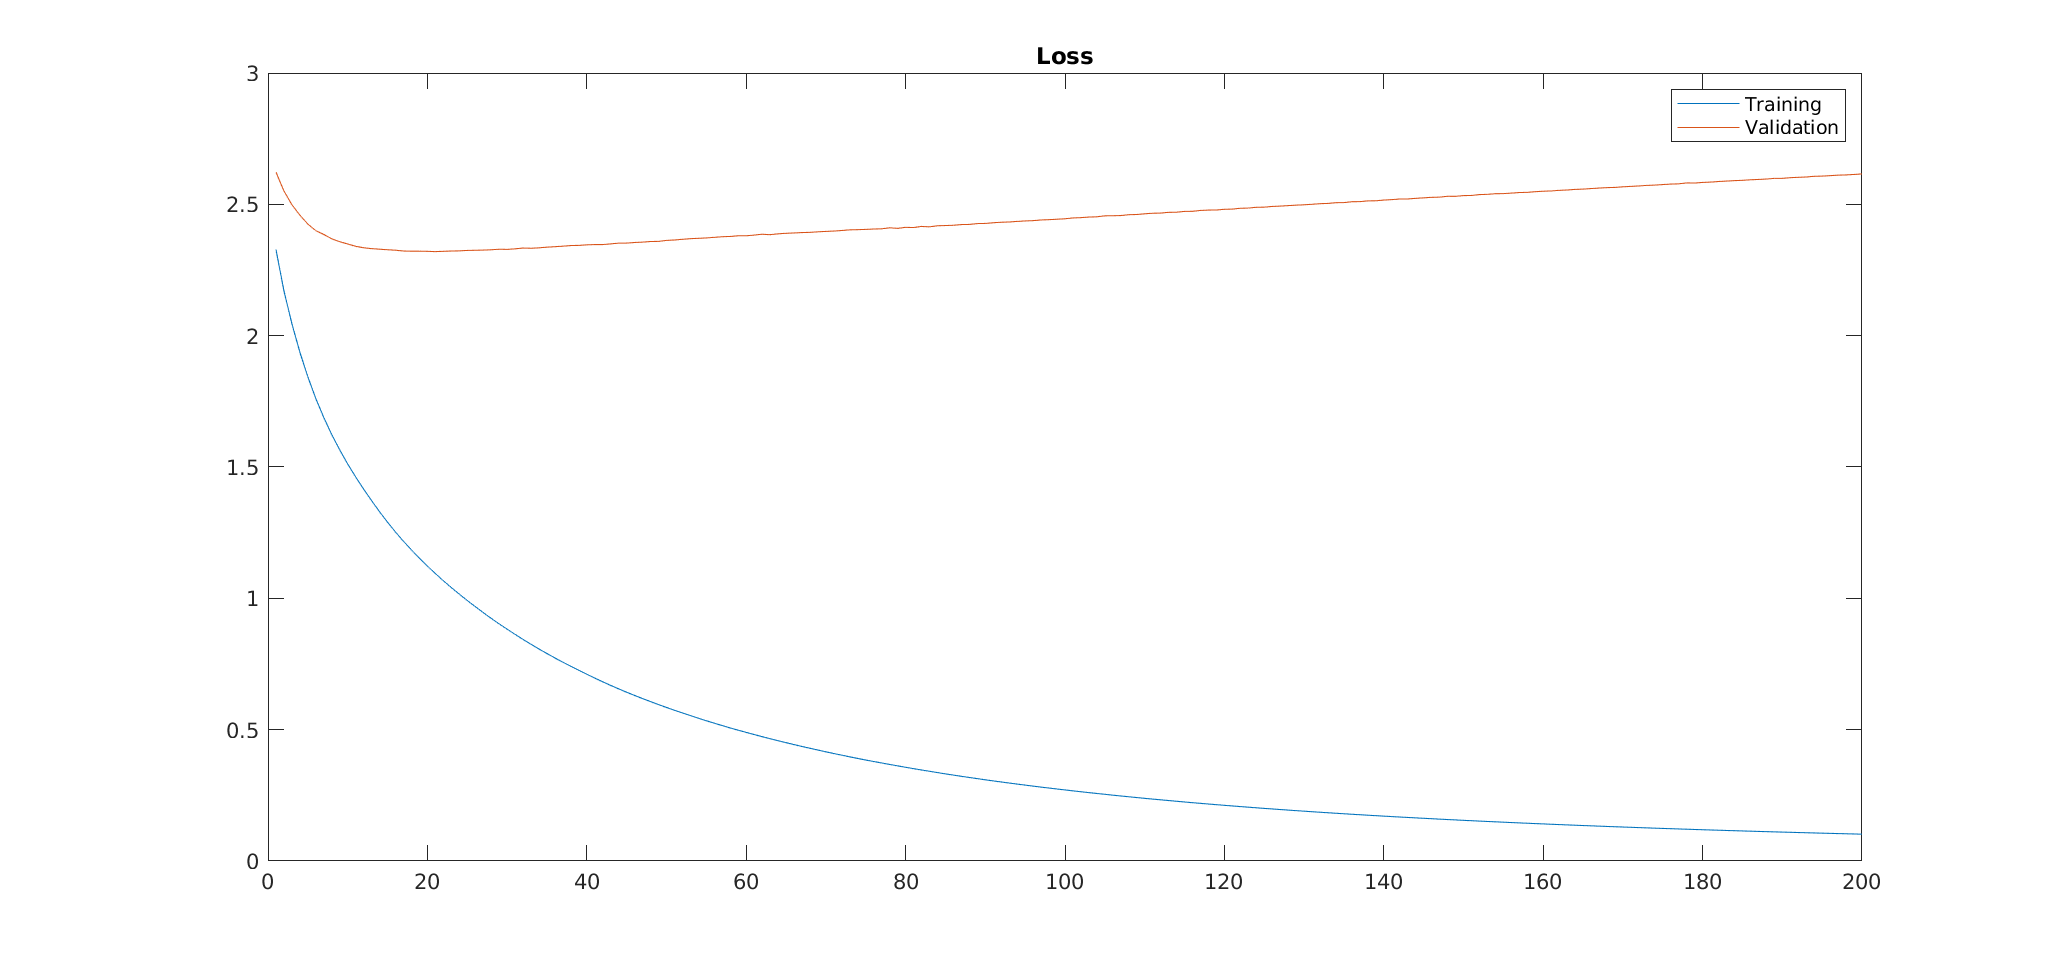
\includegraphics[width=\textwidth]{../code/result_pics/loss_sanity_overfitting.png}
        \caption{Exercise 2: sanity check, overfitting to training data}
    \end{figure}


\clearpage
\section{Exercise 3}
In exercise 3 I trained the network with  \texttt{eta\_min = 1e-5}, \texttt{eta\_max = 1e-1} and \texttt{n\_s=500}, 
\texttt{lambda = 0.01} and a batch size of 100 for 1 cycle.
Then I compared my results with the result given in the assignment instructions. I concluded that my result is similar enough and therefore 
my implementation should be correct. For the diagrams I recorded 10 values per cycle and I only used data\_batch\_1.mat for training.\\
After one cycle my network achieves a training accuracy of 60.55\%, validation accuracy of 45.62\% and a test accuracy of 46.16\%.

    \begin{figure}[ht]
        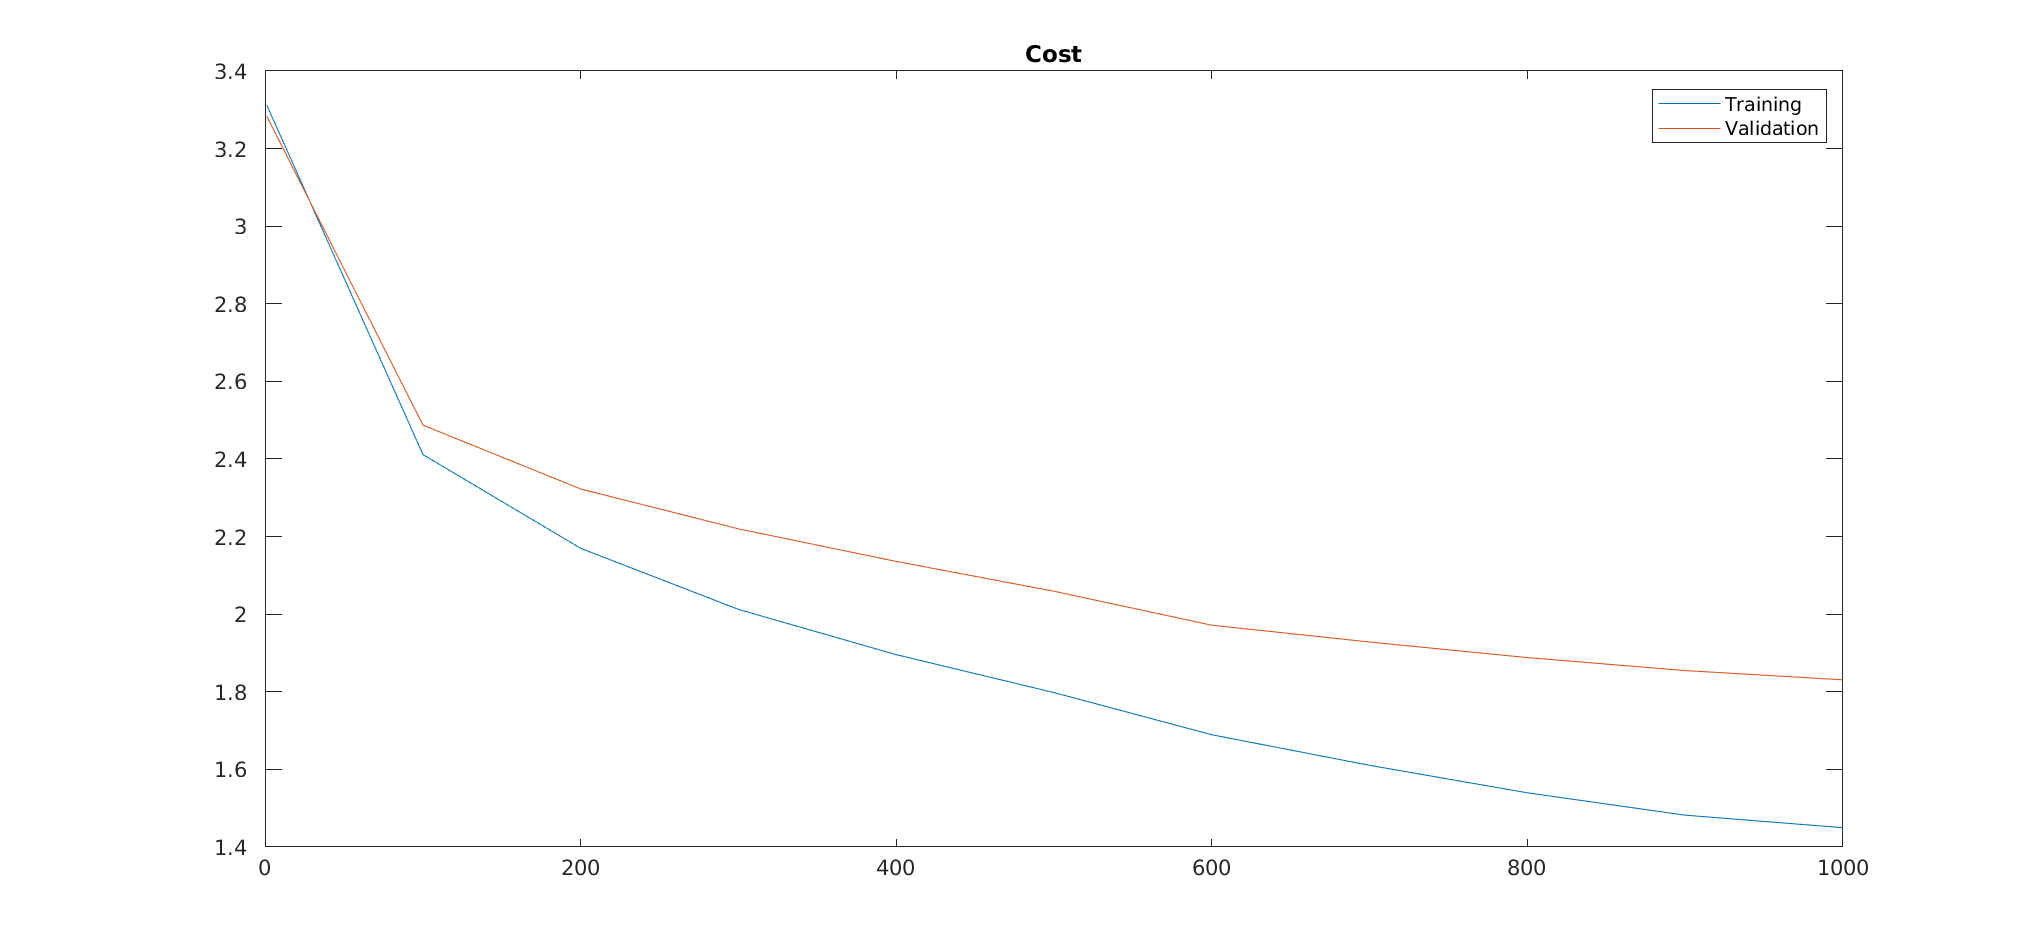
\includegraphics[width=\textwidth]{../code/result_pics/ex3_cost.png}
        \caption{Exercise 3: cost}
    \end{figure}
    \begin{figure}[ht]
        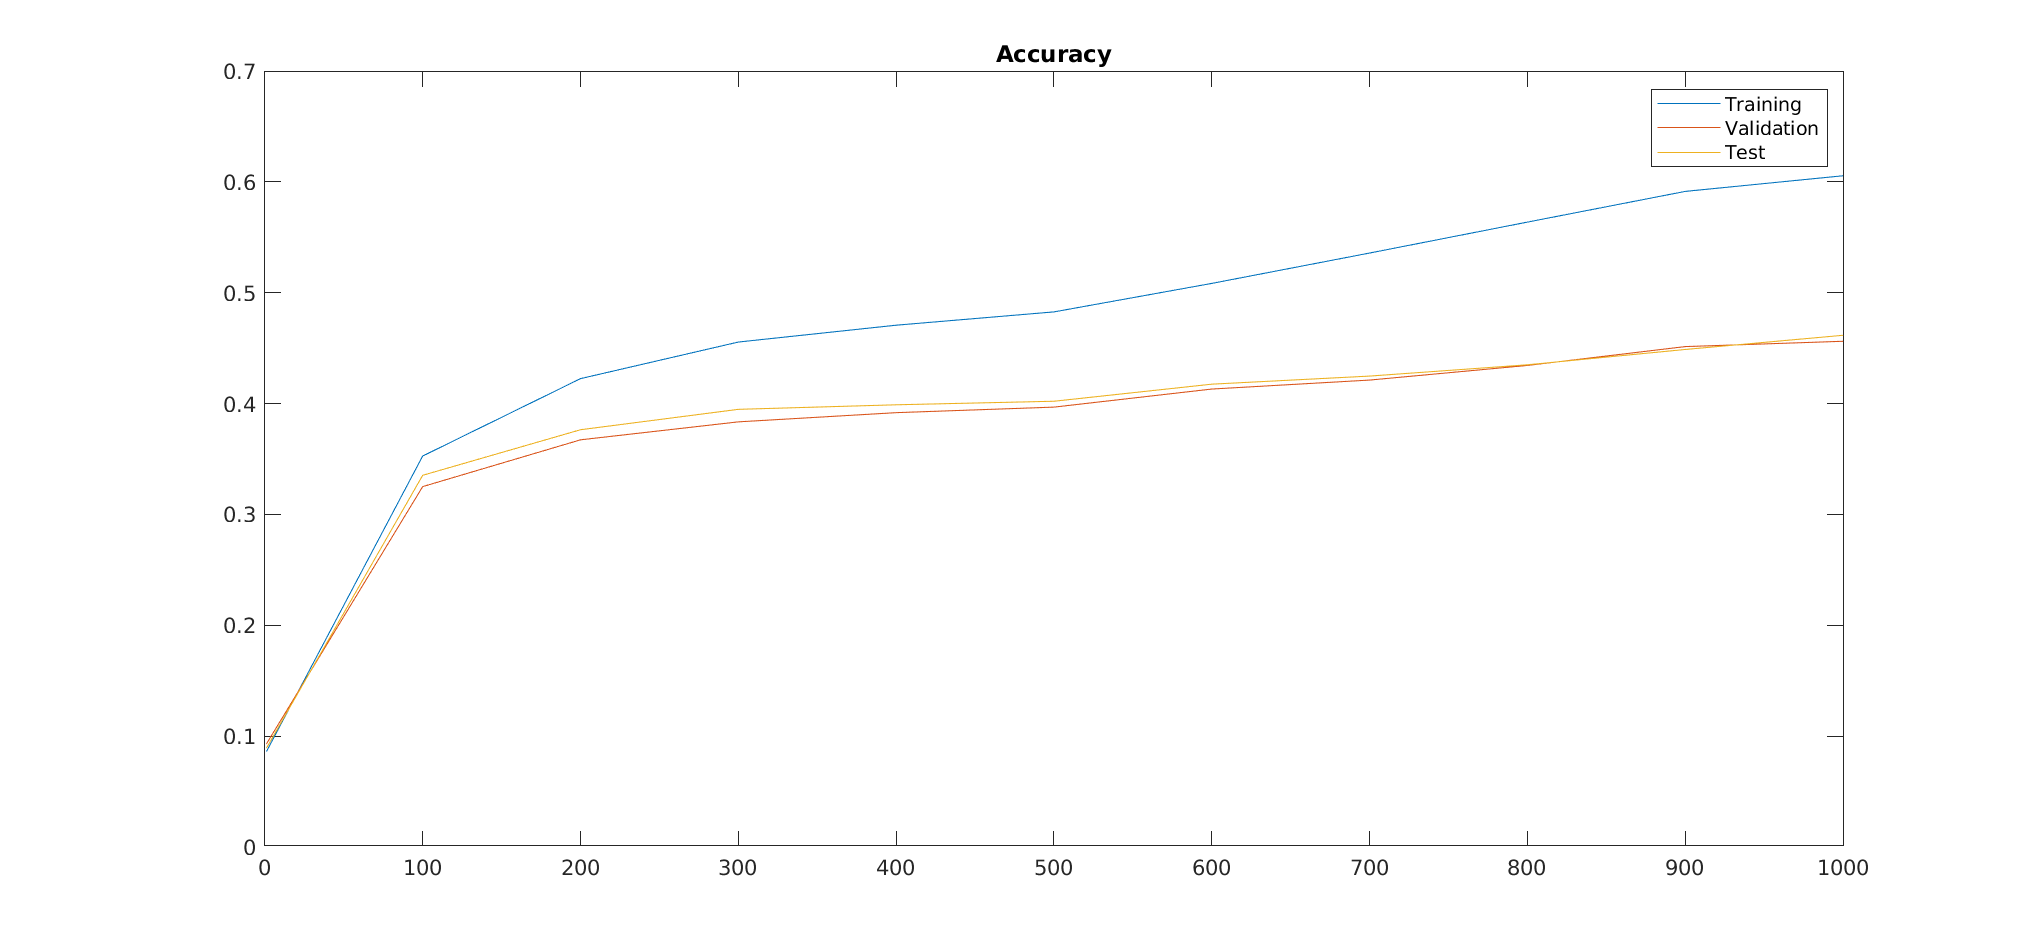
\includegraphics[width=\textwidth]{../code/result_pics/ex3_accuracy.png}
        \caption{Exercise 3: accuracy}
    \end{figure}

\clearpage

\section{Exercise 4}
\subsection{Sanity check}
For another sanity check I first ran the training with \texttt{n s=800} for 3 cycles. I got similar results as in the assignment instructions.
After 3 cycles my network achieves a training accuracy of 71.68\%, validation accuracy of 46.16\% and test accuracy of 46.88\%.
    \begin{figure}[ht]
        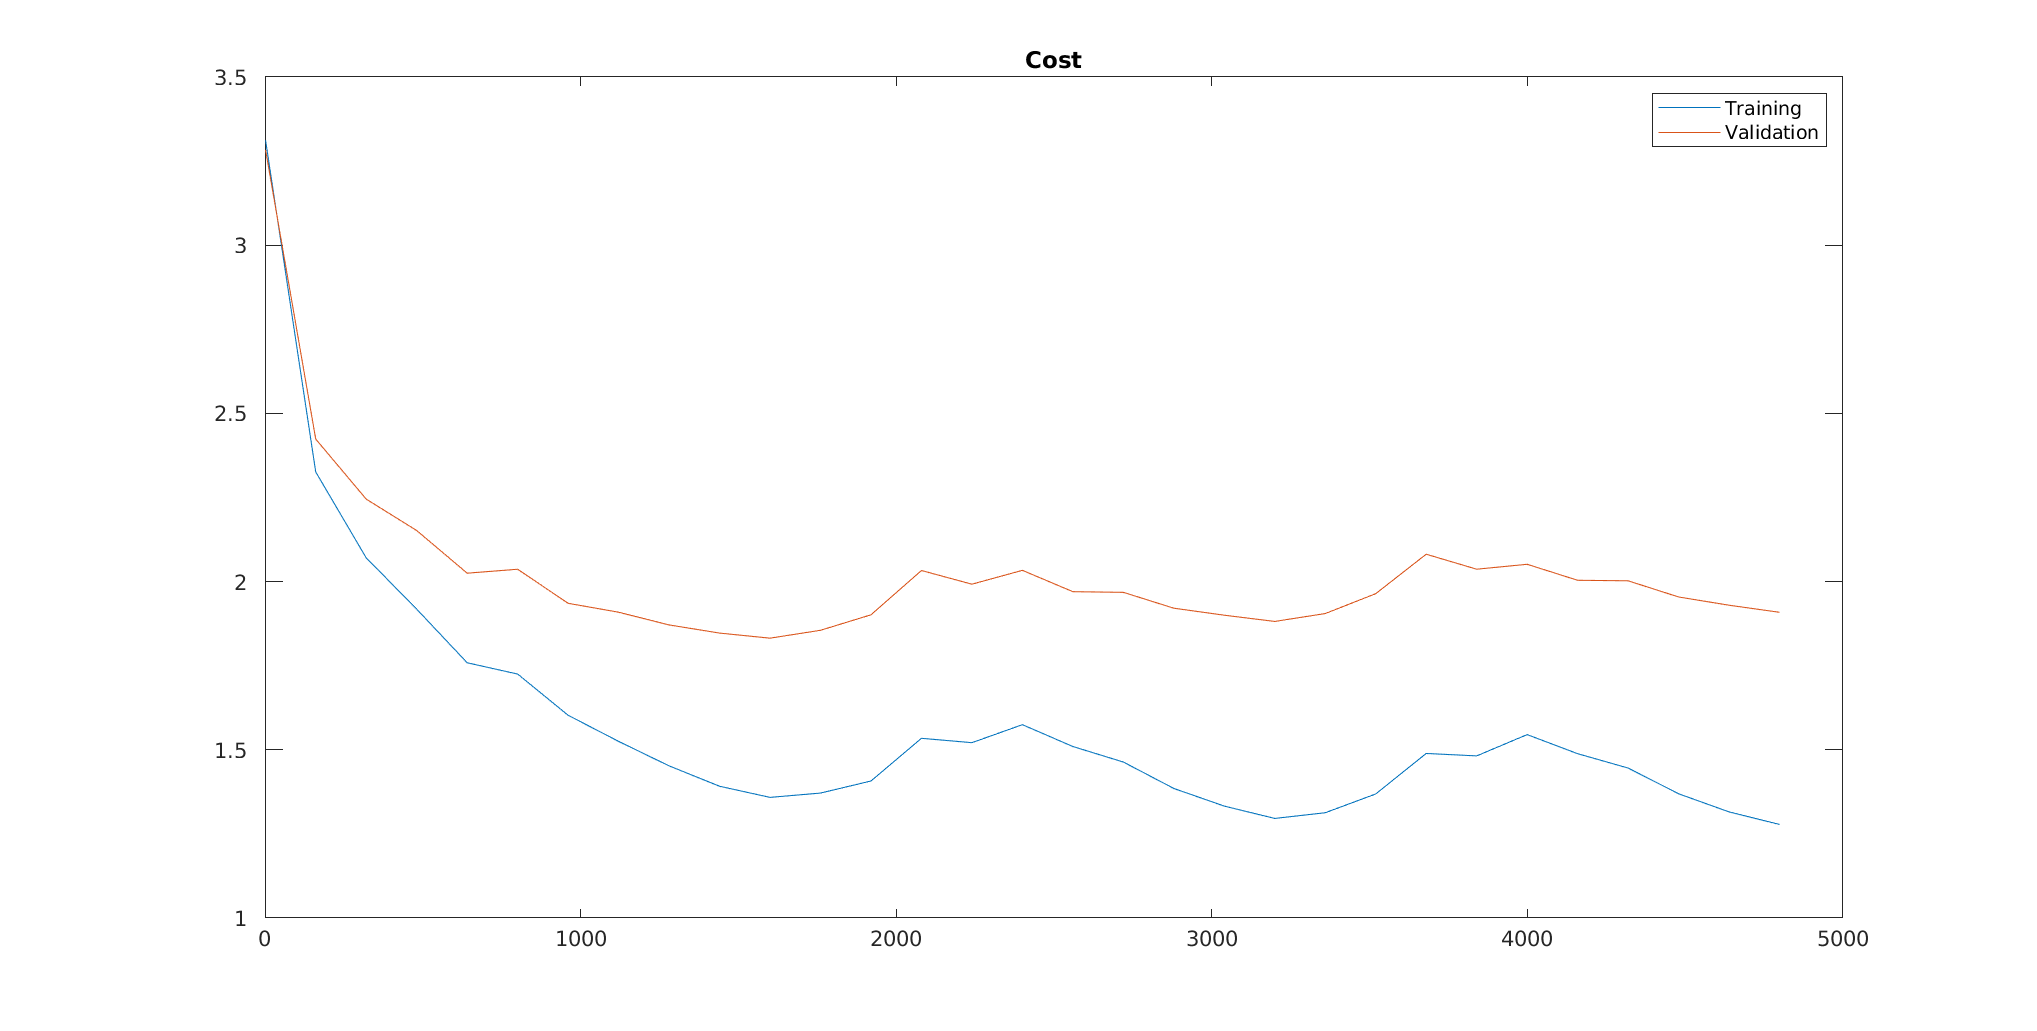
\includegraphics[width=\textwidth]{../code/result_pics/ex4_cost.png}
        \caption{Exercise 4 sanity check: cost}
    \end{figure}
    \begin{figure}[ht]
        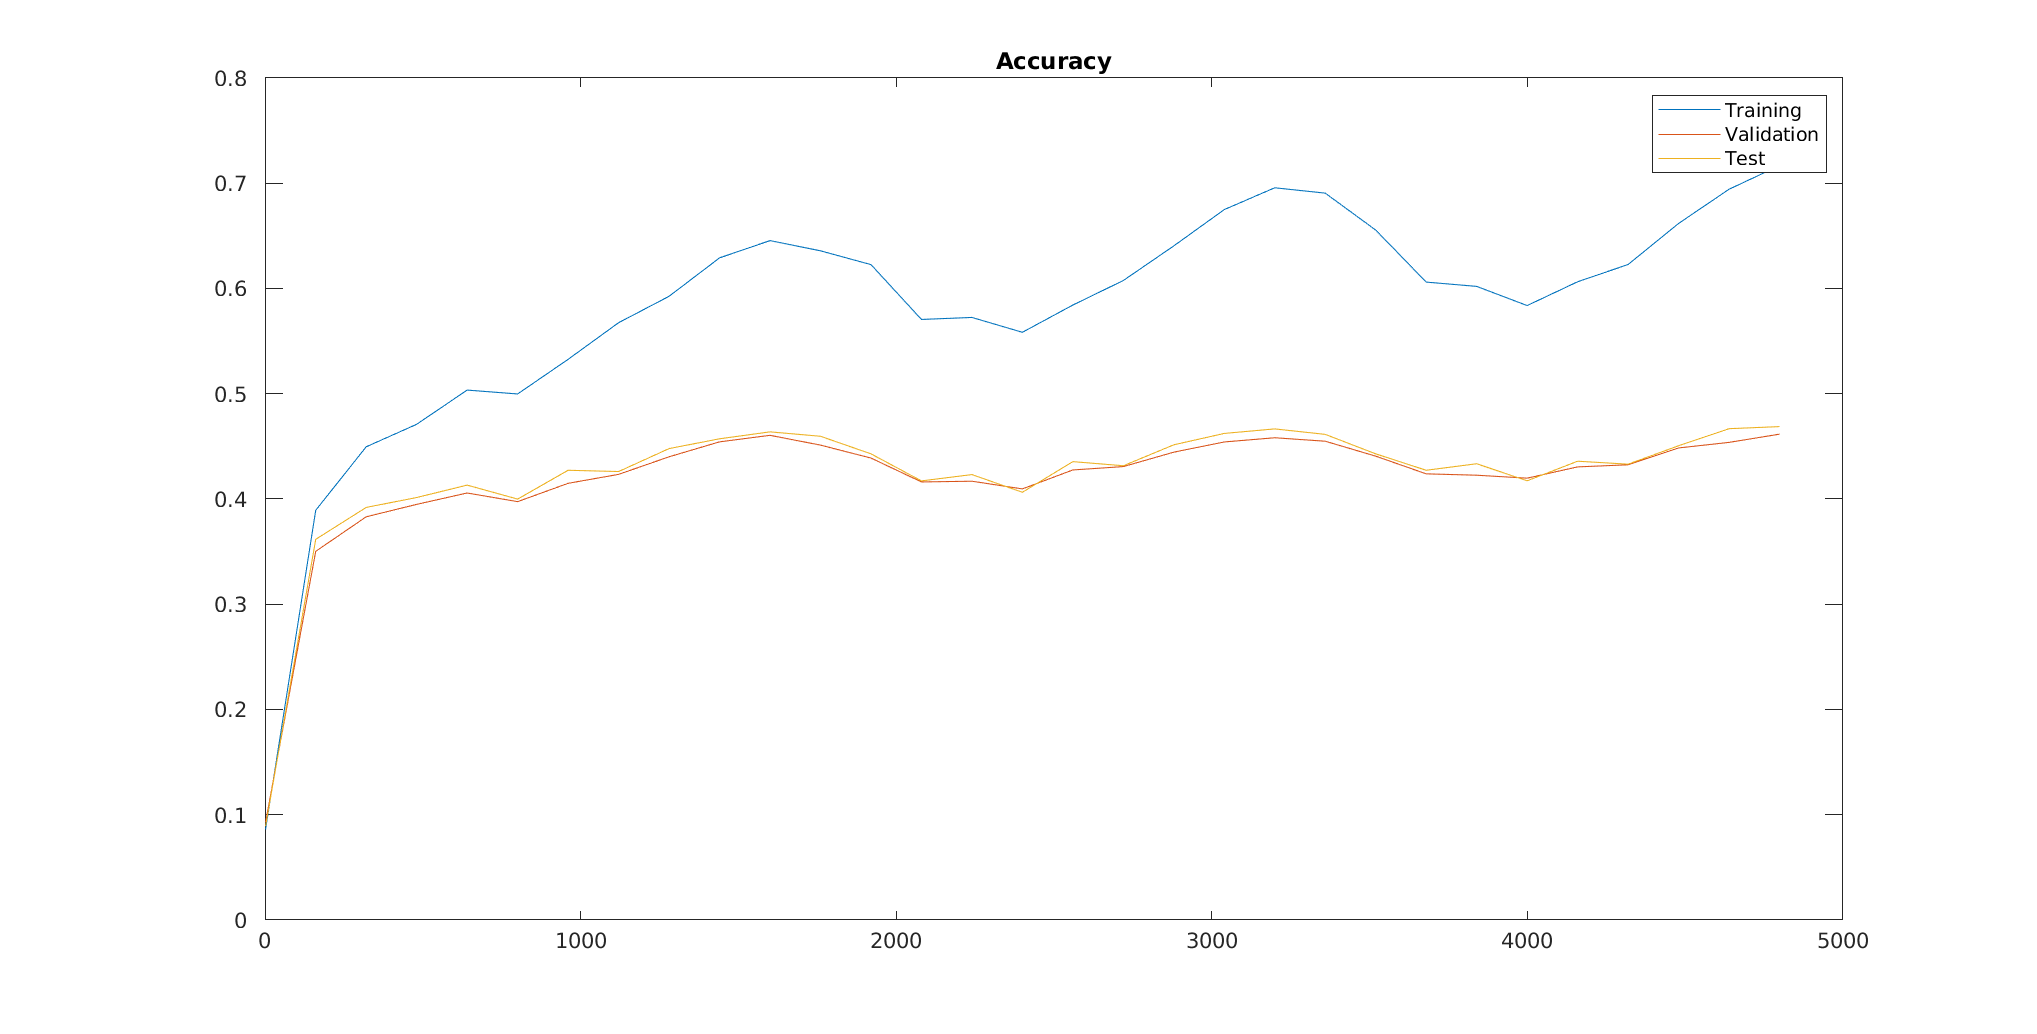
\includegraphics[width=\textwidth]{../code/result_pics/ex4_accuracy.png}
        \caption{Exercise 4 sanity check: accuracy}
    \end{figure}
\clearpage

\subsection{Lambda search}
\subsubsection{Coarse search (uniform)}
For the coarse search I sampled 20 values uniformly in the range \texttt{l\_min=0.00001} and \texttt{l\_max=0.10000}.
For each lambda I trained for 2 cycles and I used \texttt{n\_s=900}. I use all available data for training, except for 5000 that I use for validation.
    \begin{figure}[ht]
        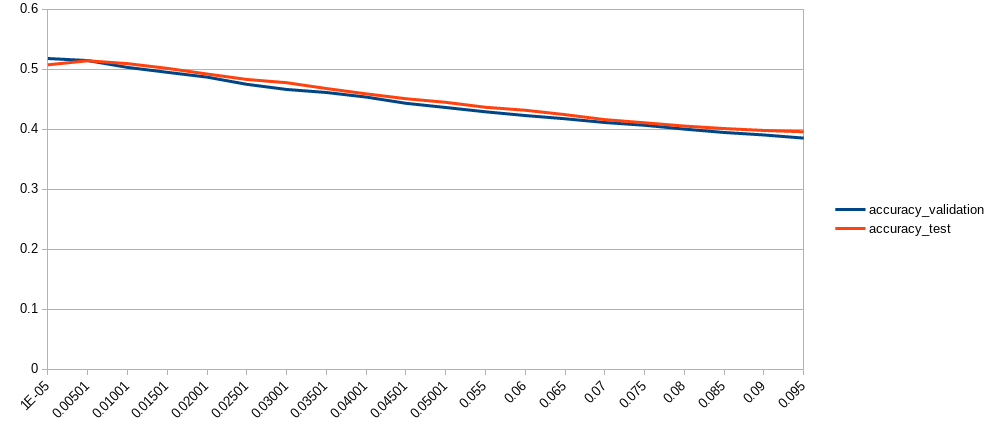
\includegraphics[width=\textwidth]{../code/result_pics/coarse_search_uniform.png}
        \caption{Exercise 4: accuracy for different lambda values, uniform coarse search}
    \end{figure}
\\
The 3 best performing networks based on the validation accuracy were achieved for
\begin{enumerate}[label=(\arabic*)]
    \item \texttt{lambda=0.00001} (51.78\%)
    \item \texttt{lambda=0.00501} (51.44\%)
    \item \texttt{lambda=0.01001} (50.30\%)
\end{enumerate}
From the graph we can see that the best results are achieved in the range \texttt{lambda=1e-5} to \texttt{lambda=1e-2}. 
Therefore I used this range for a finer, random search (see next section).

\clearpage

\subsubsection{Fine search (random)}
For the fine search I sampled 20 values randomly in the range \texttt{lambda=1e-5} to \texttt{lambda=1e-2}.
For each lambda I trained for 5 cycles and I used \texttt{n\_s=900}. I use all available data for training, except for 5000 that I use for validation.
    \begin{figure}[ht]
        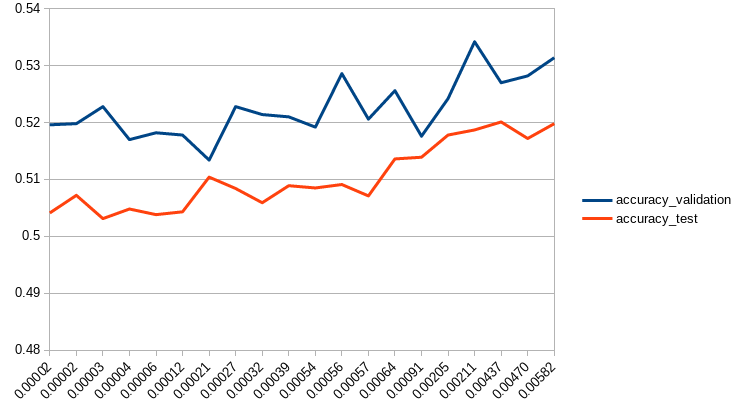
\includegraphics[width=\textwidth]{../code/result_pics/fine_search_random_1.png}
        \caption{Exercise 4: accuracy for different lambda values, random fine search}
    \end{figure}
\\
The 3 best performing networks based on the validation accuracy were achieved for
\begin{enumerate}[label=(\arabic*)]
    \item \texttt{lambda=0.00211} (53.42\%)
    \item \texttt{lambda=0.00582} (53.14\%)
    \item \texttt{lambda=0.00056} (52.86\%)
\end{enumerate}
As seen in the graph in this experiment I achieved the best results with \texttt{lambda = 0.00211}. Therefore I used this value for the training of the network.

\clearpage
\subsubsection{Training with best lambda}
For the final training I used all available data for training, except 1000 that I use for validation.
The lambda search resulted in the best performance when using \texttt{lambda = 0.00211}, so this value is used for the final training.
I ran the training with 2 different values for n\_s and for 3 cycles. 
\begin{enumerate}[label=(\arabic*)]
    \item \texttt{n\_s=900}: test accuracy: 51.54\% 
    \item \texttt{n\_s=980}: test accuracy: 51.91\%
\end{enumerate}
Below are the resulting diagrams for \texttt{n\_s=980}, since it gave a slightly better result.
    \begin{figure}[ht]
        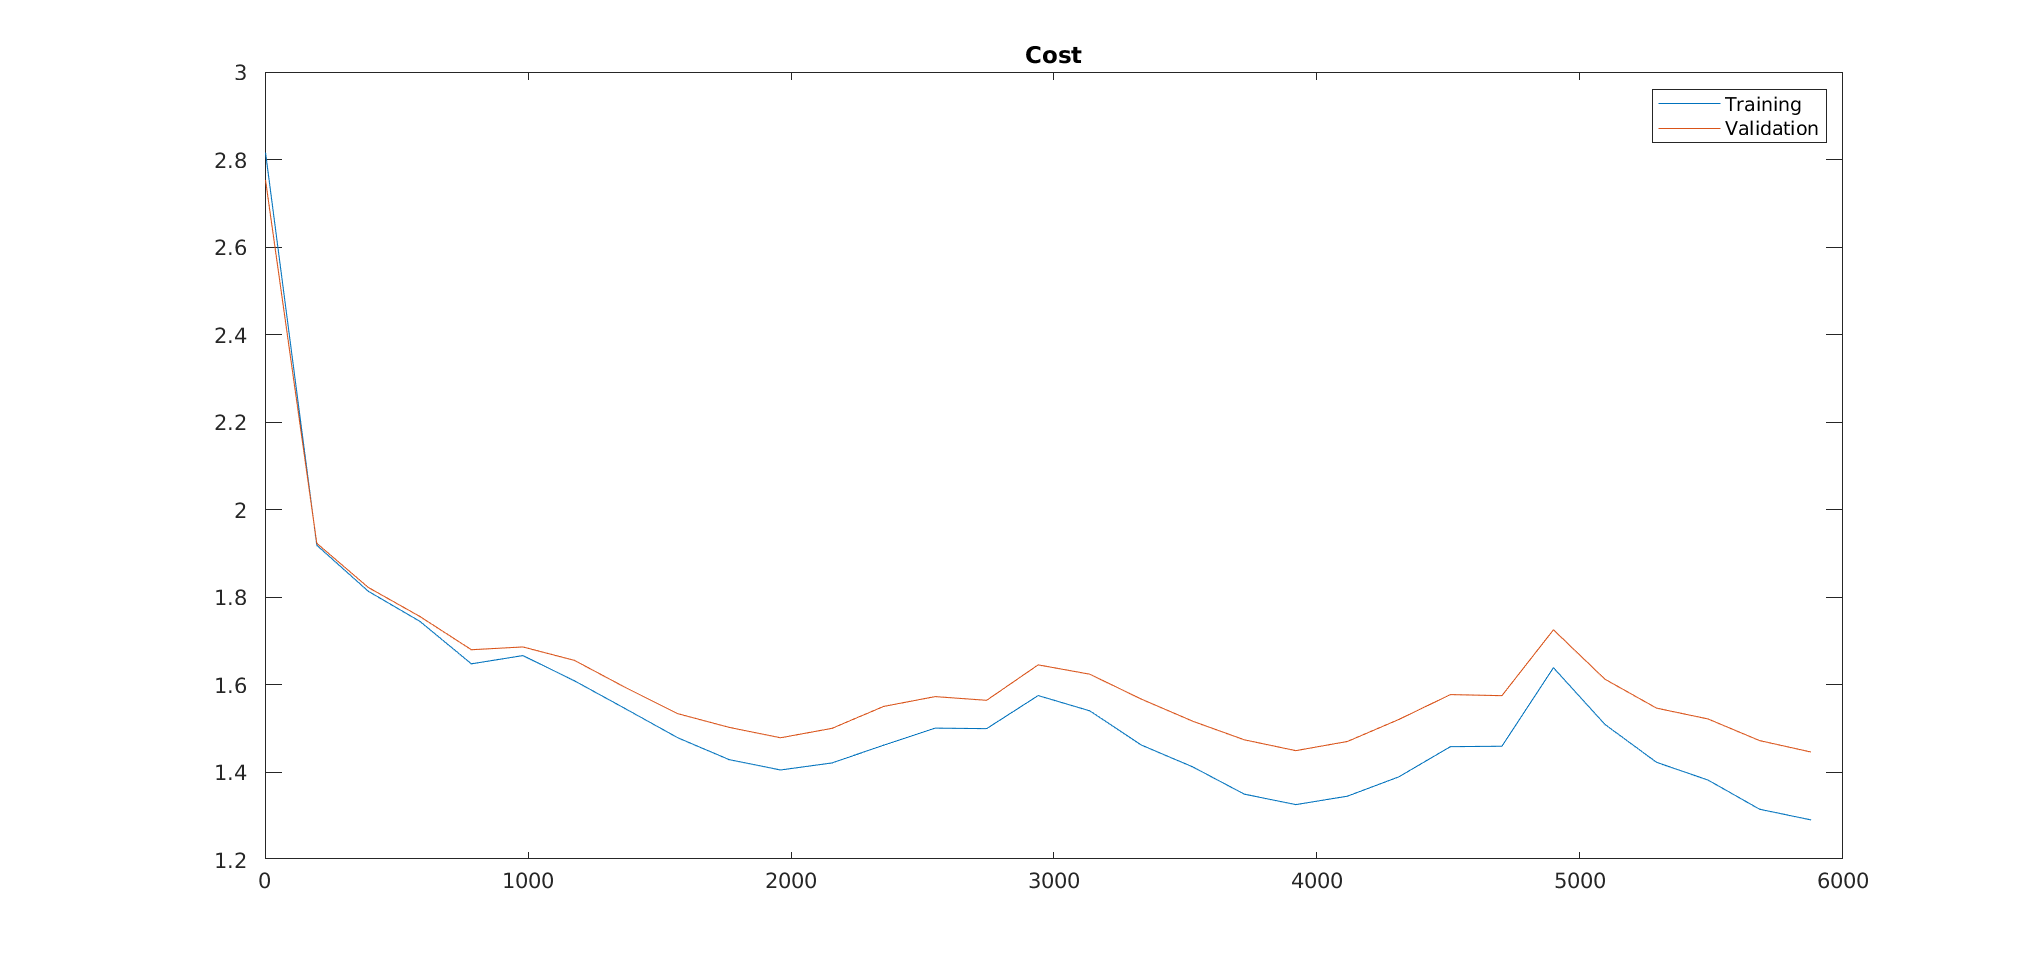
\includegraphics[width=\textwidth]{../code/result_pics/cost_lambda=0.00211_ns=980_cycles=3.png}
        \caption{Exercise 4: final training}
    \end{figure}
    \begin{figure}[ht]
        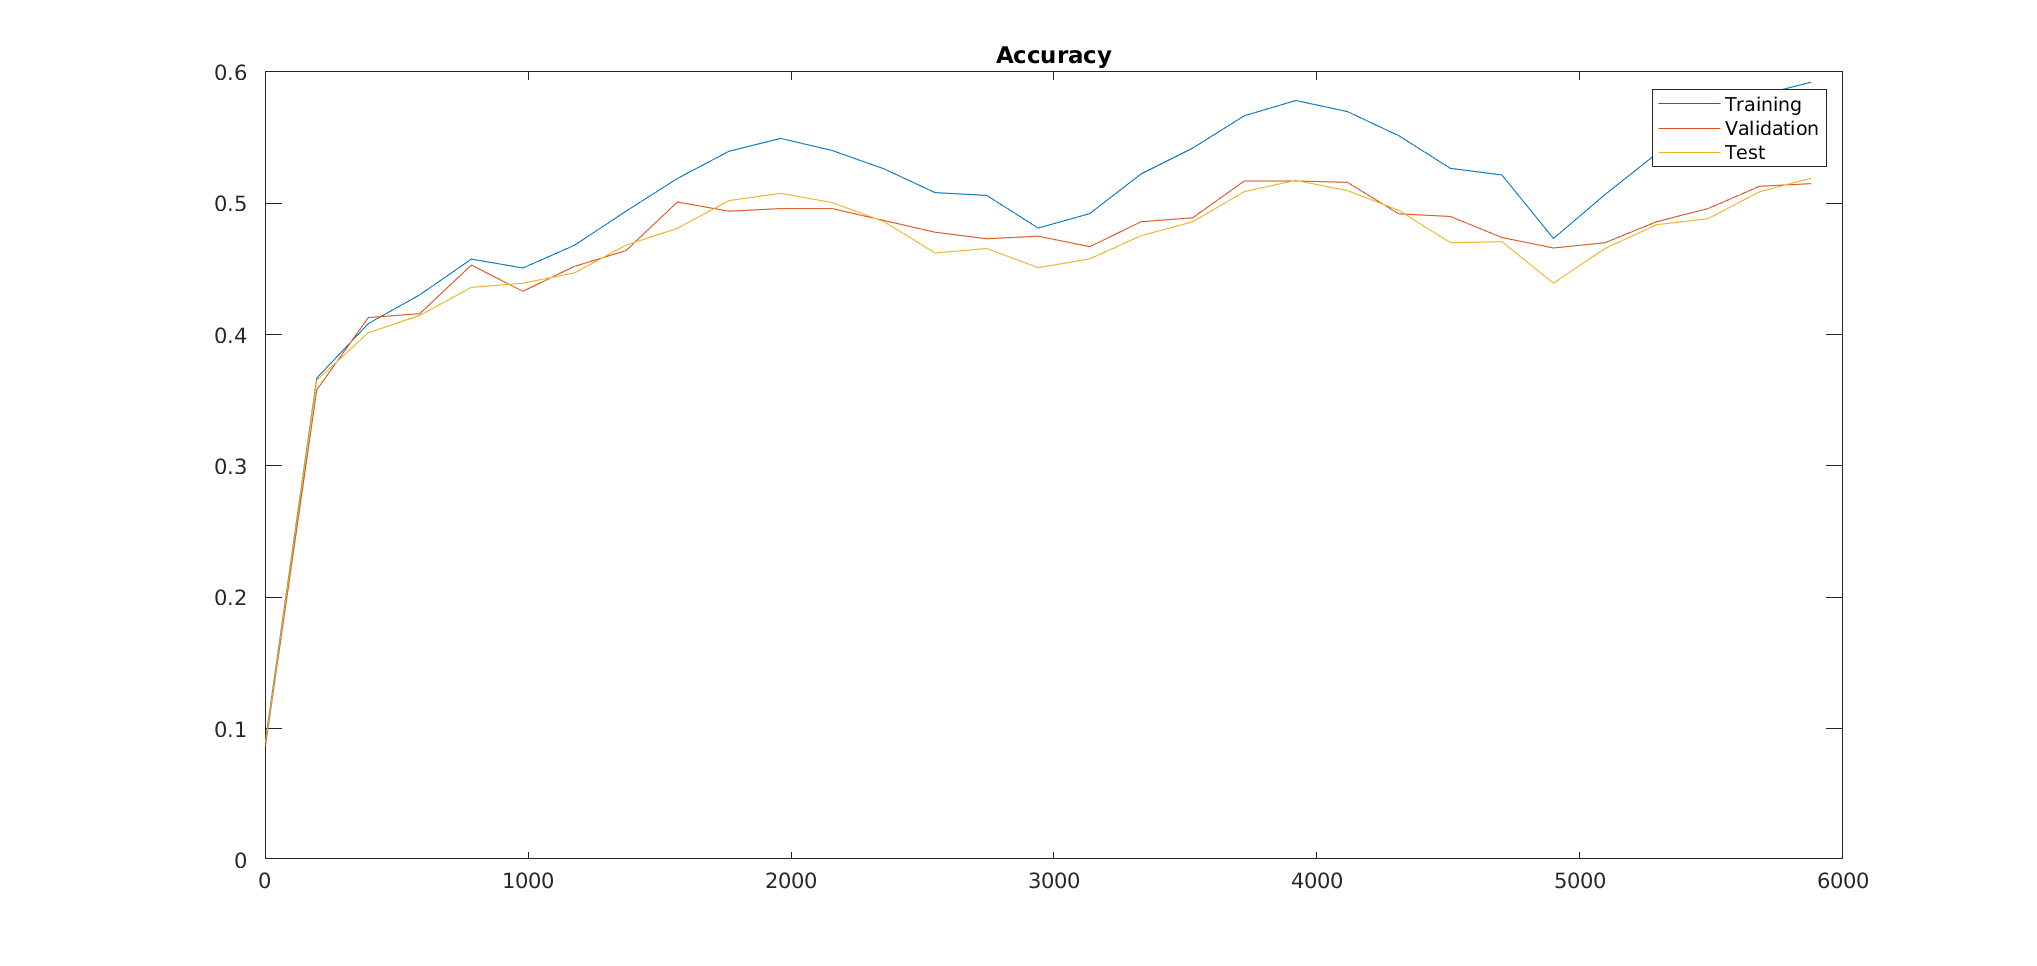
\includegraphics[width=\textwidth]{../code/result_pics/accuracy_lambda=0.00211_ns=980_cycles=3.png}
        \caption{Exercise 4: final training}
    \end{figure}
\clearpage
The final performance is 
\begin{itemize}
    \item training accuracy: 59.22\%
    \item validation accuracy: 51.5\%
    \item test accuracy: 51.91\%
\end{itemize}
